\documentclass[addpoints]{exam}
\usepackage{preamble}
\sisetup{group-separator = {,}}

\pagestyle{headandfoot}
\runningheadrule

\firstpagefooter{Access for free at \href{https://openstax.org/books/astronomy-2e/pages/1-introduction}{https://openstax.org/books/astronomy-2e/pages/1-introduction}}{}{}
\runningfooter{Access for free at \href{https://openstax.org/books/astronomy-2e/pages/1-introduction}{https://openstax.org/books/astronomy-2e/pages/1-introduction}}{}{}

\firstpageheader{Astronomy}{Test}{Chapter 4: {\small Earth, Moon \& Sky}}


\CorrectChoiceEmphasis{\color{red}\bfseries}
\SolutionEmphasis{\color{red}}
\printanswers

\begin{document}
\begin{questions}

\question 
Why are the winter months so cold in Texas? Explain this from an astronomical perspective.
\qspace

\question %5
What are the two ways that the tilt of Earth's axis causes the summers in the United States to be warmer than the winters?
\qspace

\question %21
The term equinox translates as ``equal night.'' Explain why this translation makes sense from an astronomical point of view.
\qspace

\question %22
The term solstice translates as ``Sun stop.'' Explain why this translation makes sense from an astronomical point of view.
\qspace

\question %24
When Earth's Northern Hemisphere is tilted toward the Sun during June, some would argue that the cause of our seasons is that the Northern Hemisphere is physically closer to the Sun than the Southern Hemisphere, and this is the primary reason the Northern Hemisphere is warmer. What argument or line of evidence could contradict this idea?
\qspace

\question %26
In countries at far northern latitudes, the winter months tend to be so cloudy that astronomical observations are nearly impossible. Why can't good observations of the stars be made at those places during the summer months?
\qspace

\question
What would change if the Earth had a no tilt instead of a \SI{23.5}{\degree} tilt?
\qspace

% \begin{choices}
% \correctchoice There would be no changes in season
% \end{choices}


\section*{4.7 Eclipses of the Sun and Moon}

\question
What are some differences between lunar and solar eclipses?

\question %8
What is the phase of the Moon during a total solar eclipse? During a total lunar eclipse?

\question %15
Why don't lunar eclipses happen during every full moon?

\question %28
A car accident occurs around midnight on the night of a full moon. The driver at fault claims he was blinded momentarily by the Moon rising on the eastern horizon. Should the police believe him?


% \question
% Which territory would be the LAST in the world to welcome the new year on January 1?

% \begin{figure}[h!]
%     \centering
%     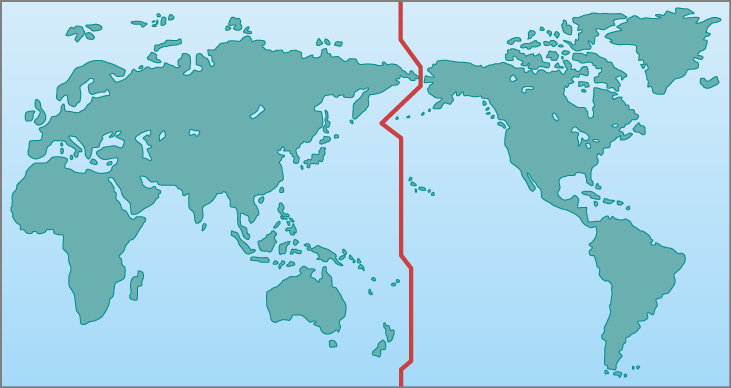
\includegraphics[width=2.5in]{Figures/Figure4.11.jpg}
%     %\caption{Caption}
%     %\label{fig:my_label}
% \end{figure}

% \begin{choices}
% \choice Russia  
% \choice South America
% \correctchoice Alaska
% \choice Australia
% \end{choices}

% \question
% Stonehenge, the ancient monument in England, was used to \fillin[][2in]\ .

% \begin{figure}[h!]
%     \centering
%     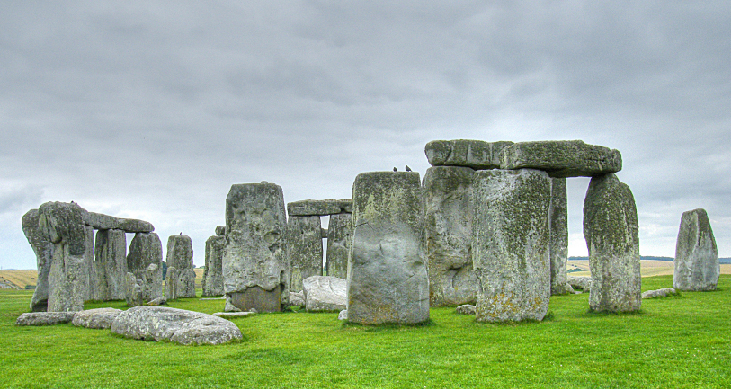
\includegraphics[width=2.5in]{Figures/Figure4.12.jpg}
%     \caption*{\small Credit: modification of work by Adriano Aurelio Araujo}
%     % \label{fig:my_label}
% \end{figure}

% \begin{choices}
% \choice measure the circumference of Earth
% \correctchoice keep track of the motions of the Sun and Moon
% \choice track the location of Neptune
% \choice climb to get a better view of the sky
% \end{choices}



\question %1
Discuss how \textbf{latitude} and \textbf{longitude} on Earth are similar to \textbf{declination} and \textbf{right ascension} in the sky.

\question %2
What is the latitude of the North Pole? The South Pole? Why does longitude have no meaning at the North and South Poles?

\question %9
On a globe or world map, find the nearest marked latitude line to your location. Is this an example of a great circle? Explain.

\question
What causes night and day? Explain this from an astronomical persepctive.

\question %11
What is the origin of the terms ``a.m.'' and ``p.m'' in our timekeeping?

\question %36
What is the right ascension and declination of the vernal equinox?

\question %37
What is the right ascension and declination of the autumnal equinox?

\question %38
What is the right ascension and declination of the Sun at noon on the summer solstice in the Northern Hemisphere?

\question
What must be the latitude of a city where the Sun crosses the zenith at noon on June 21?

\begin{solution}
About \SI{23}{\degree} North, same as the axial tilt of the Earth. This location is, by definition, called the Topic of Cancer.
\end{solution}

\question %52
What is the altitude of the Sun at noon on December 22, as seen from a place on the Tropic of Cancer?

% \question
% What is the meridian?

% \begin{choices}
%     \correctchoice a great circle on the celestial sphere
% \end{choices}

% \question
% What is declination?

% \question
% What is right ascension?

% \question
% A solar day is \fillin\ .

% \question
% Which of the following is the best celestial point to mark the time elapsed in 1 solar day?

% \begin{choices}
%     \choice where the Sun sets in the West
%     \correctchoice where the Sun crosses the meridian
%     \choice where the Sun rises in the East
%     \choice where the Sun crosses the celestial equator
% \end{choices}

% \question
% 3 revolutions of Earth around the Sun takes \fillin\ .

% \begin{choices}
% \choice 3 days
% \choice 3 weeks
% \choice 3 months
% \correctchoice 3 years 
% \end{choices}

% \question
% 21 rotations of Earth on its axis takes \fillin\ .

% \begin{choices}
% \choice 21 hours
% \correctchoice 21 days
% \choice 21 years
% \choice 21 weeks
% \end{choices}

\question
What is the tilt of Earth's axis?

\begin{choices}
    \correctchoice \SI{23.5}{\degree}
    \choice \SI{45}{\degree}
    \choice \SI{21}{\degree}
    \choice \SI{0}{\degree}
\end{choices}

\question
Here in Texas, we live in Earth's \fillin\ hemisphere.

\begin{choices}
    \choice Southern
    \correctchoice Northern
    \choice Eastern
    \choice Western
\end{choices}

\question
Why are the summer months in Texas so hot?

\begin{choices}
    \choice Earth is much closer to the Sun in the summer
    \correctchoice the northern hemisphere is tilted towards the Sun, absorbing more daily sunlight
    \choice people are more active, causing body heat to dissipate throughout the environment
    \choice during the summer the Sun becomes hotter and brighter for a few months
\end{choices}

\question
Which figure below could represent the Southern Hemisphere (e.g., Argentina) in June?

\question 
Which figure below could represent the Northern Hemisphere (e.g., Texas) in June?

\question
Which figure could represent Australia in December?

\question
Which figure could represent Boston in December?

\begin{figure}[h!]
    \centering
    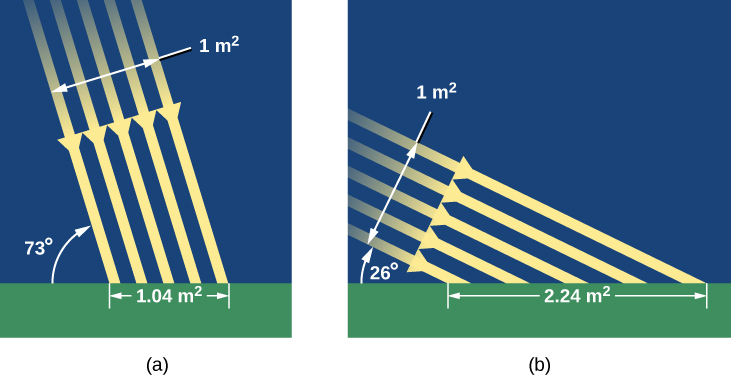
\includegraphics{Figures/Figure4.6.jpg}
    % \caption{Caption}
    % \label{fig:my_label}
\end{figure}

\clearpage

\question
Which of the following is NOT a reason why summer months are hotter in the Northern Hemisphere?

\begin{choices}
    \choice Sunlight strikes northern countries more directly
    \correctchoice Earth is 3\% closer to the Sun on June 21
    \choice The Sun is visible for more time
    \choice Earth's southern hemisphere is tilted away from the Sun
\end{choices}

\question
Which astronomical event is depicted in the figure below?

\begin{minipage}{0.4\textwidth}
    \centering
    \begin{choices}
    \choice Winter solstice (December 21)
    \choice Spring Equinox (March 21)
    \correctchoice Summer solstice (June 21)
    \choice Fall Equinox\\ (September 21)
    \end{choices}
\end{minipage}%
\begin{minipage}{0.5\textwidth}
    \centering
    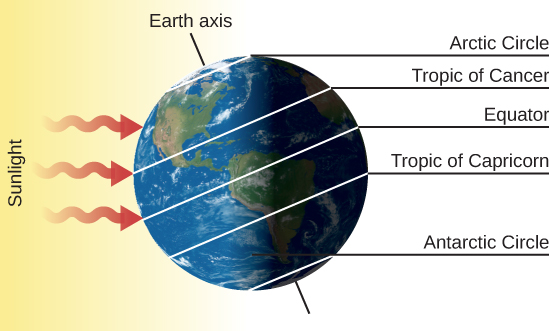
\includegraphics[width=1.5in]{Figures/Figure4.8.jpg}
\end{minipage}
\vspace{1em}

\question
Which astronomical event is depicted in the figure below?

\begin{minipage}{0.45\textwidth}
    \centering
    \begin{choices}
    \choice Spring Equinox\\ (March 21)
    \choice Fall Equinox\\ (September 21)
    \choice Summer Solstice\\ (June 21)
    \correctchoice Winter Solstice\\ (December 21)
    \end{choices}
\end{minipage}%
\begin{minipage}{0.5\textwidth}
    \centering
    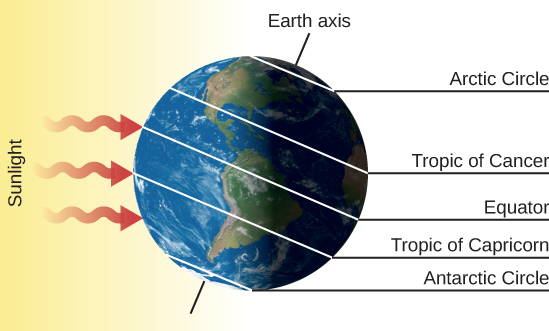
\includegraphics[width=1.5in]{Figures/Figure4.9.jpg}
\end{minipage}
\vspace{1em}

\question
The Tropic of Cancer is at latitude \fillin[][1cm]\ .

\begin{choices}
    \correctchoice \SI{23}{\degree N}
    \choice \SI{0}{\degree} (Equator)
    \correctchoice \SI{23}{\degree S}
    \correctchoice \SI{45}{\degree W}
\end{choices}

\question
If you travel to a place on the Tropic of Cancer (e.g., Hawaii) on the summer solstice, you'll observe that the Sun at noon \ldots

\begin{choices}
    \choice crosses the constellation of Cancer
    \correctchoice is at your zenith (directly overhead)
    \choice reaches its lowest point in the sky
    \choice gets blocked by the Moon
\end{choices}

% \question
% Why is the International Date Line where located where Earth's surface is mostly water?

% \begin{figure}[h!]
%     \centering
%     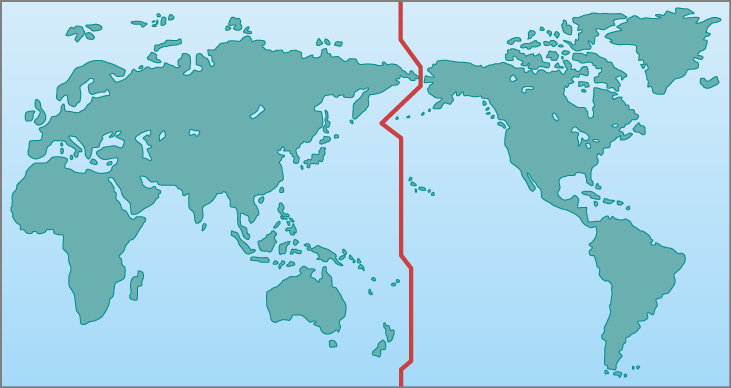
\includegraphics[width=2.5in]{Figures/Figure4.11.jpg}
%     %\caption{Caption}
%     %\label{fig:my_label}
% \end{figure}

% \begin{choices}
% \correctchoice So that neighboring countries do not have different days.
% \choice Benjamin Franklin wanted it that way.
% \choice This location is where the Sun is brightest throughout the year.
% \choice There's no good reason.
% \end{choices}

% \question
% \fillin\ are known as phases of the moon.

\question
Which phenomenon is represented in the figure below?
\vspace{1em}

\begin{minipage}{0.45\textwidth}
    \centering
    \begin{choices}
    \choice lunar eclipse
    \choice supernova
    \correctchoice solar eclipse
    \choice retrograde motion
    \end{choices}
\end{minipage}%
\begin{minipage}{0.5\textwidth}
    \centering
    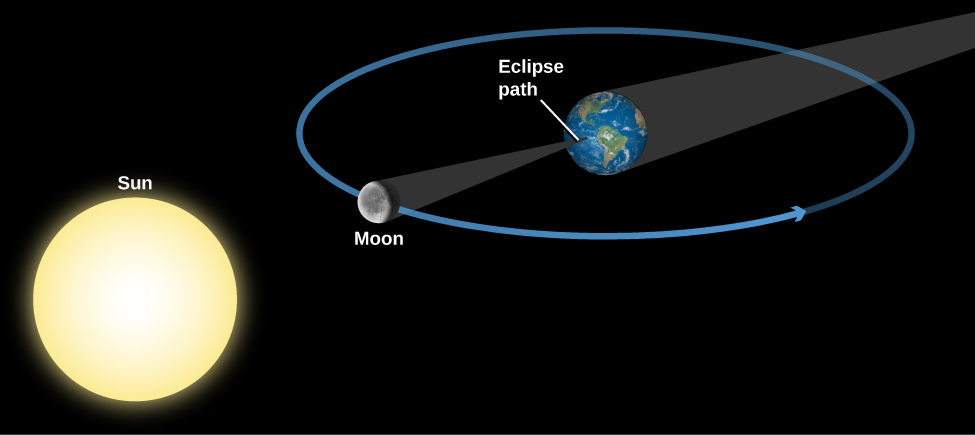
\includegraphics[width=2.5in]{Figures/Figure4.22.jpg}
\end{minipage}
\vspace{1em}

\question
Which part of the Sun may be seen during a solar eclipse? (Warning: never look directly at the Sun).

\begin{choices}
    \choice the core
    \choice the photosphere
    \choice the surface
    \correctchoice the corona (outer atmosphere)
\end{choices}

\question
How long does viewing a solar eclipse last?

\begin{choices}
    \choice about 1 hour
    \correctchoice no more than 7 minutes
    \choice 7 days
    \choice 1 month
\end{choices}



% \question
% What is a solar eclipse?

% \question
% \fillin\ is known as a lunar eclipse.

\question
Which phenomenon is represented in the figure below?
\vspace{1em}

\begin{minipage}{0.45\textwidth}
    \centering
    \begin{choices}
    \correctchoice lunar eclipse
    \choice supernova
    \choice solar eclipse
    \choice hypernova
    \end{choices}
\end{minipage}%
\begin{minipage}{0.5\textwidth}
    \centering
    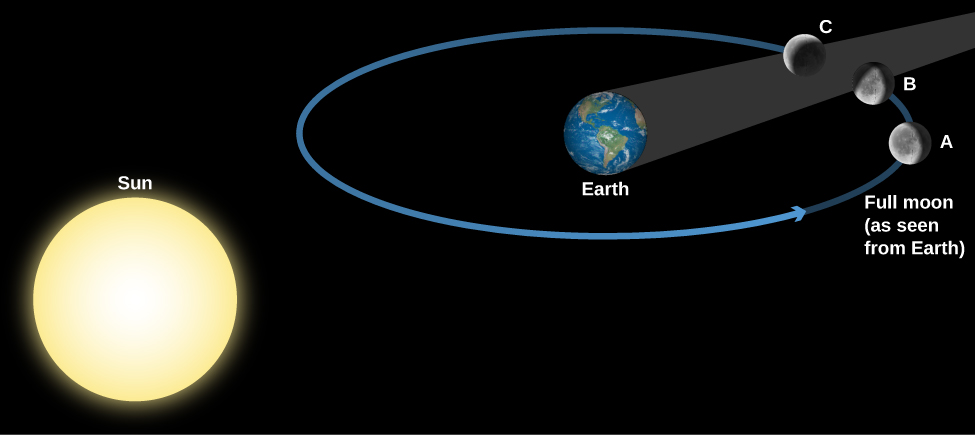
\includegraphics[width=3in]{Figures/Figure4.24.jpg}
\end{minipage}

\question
What happens during a lunar eclipse?

\begin{choices}
    \choice The Moon blocks sunlight on Earth's surface.
    \choice The Moon's atmosphere reflects sunlight, turning it ``blood'' orange.
    \choice The Sun and Moon collide.
    \correctchoice The Earth blocks sunlight on the Moon's surface.
\end{choices}

\question
Why don't lunar and solar eclipses happen every month?

\begin{choices}
    \correctchoice The \SI{5}{\degree} tilt of the Moon's orbit usually prevents the Earth and Moon from crossing each others' shadows.
    \choice The Sun isn't always bright enough to make eclipses happen.
    \choice Eclipses only happen when at least 3 planets in the solar system align.
    \choice They do happen every month; we just can't see them in Texas all the time.
\end{choices}

\question 
What causes the Moon to turn ``blood'' orange during a lunar eclipse?

\begin{choices}
    \choice The Moon's atmosphere absorbs red wavelengths from the Sun.
    \choice The Moon's true orange surface is made visible during an eclipse.
    \correctchoice Earth's atmosphere focuses the redder wavelengths of light on the Moon (like during a sunset).
    \choice The orange light from Mars reflects off the Moon
\end{choices}

\question
What is the tilt of Earth's axis relative to its orbit around the Sun?

\begin{choices}
    \correctchoice \SI{23.5}{\degree}
    \choice \SI{45}{\degree}
    \choice \SI{21}{\degree}
    \choice \SI{0}{\degree}
\end{choices}

\question
Here in Texas, we live in Earth's \fillin\ hemisphere.

\begin{choices}
    \choice Southern
    \correctchoice Northern
    \choice Eastern
    \choice Western
\end{choices}

\question
Why are the summer months in Texas so hot?

\begin{choices}
    \choice Earth is much closer to the Sun in the summer
    \correctchoice the northern hemisphere is tilted towards the Sun, absorbing more daily sunlight
    \choice people are more active, causing body heat to dissipate throughout the environment
    \choice during the summer the Sun becomes hotter and brighter for a few months
\end{choices}

\question
The figures below represent direct (a) and indirect (b) sunlight. Which figure could represent the Antarctica (latitude \SI{80}{\degree}\,S) June?

\question 
The figures below represent direct (a) and indirect (b) sunlight. Which figure could represent a city at latitude \SI{56}{\degree}\,N in June?

\question
The figures below represent direct (a) and indirect (b) sunlight. Which figure could represent South Africa (latitude \SI{30}{\degree}\,S) in December?

\begin{figure}[h!]
    \centering
    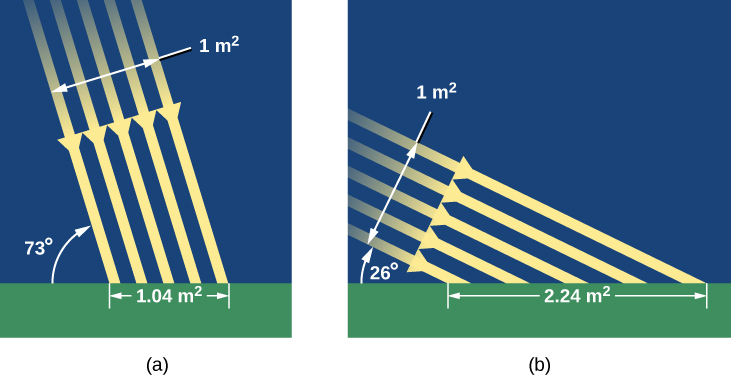
\includegraphics{Figures/Figure4.6.jpg}
\end{figure}

\clearpage

\question
Which of the following is NOT a reason why summer months are hotter in the Northern Hemisphere?

\begin{choices}
    \choice Sunlight strikes northern countries more directly
    \correctchoice Earth is 3\% closer to the Sun on June 21
    \choice The Sun is visible for more time
    \choice Earth's southern hemisphere is tilted away from the Sun
\end{choices}

\question
Which astronomical event is depicted in the figure below?

\begin{minipage}{0.45\textwidth}
    \centering
    \begin{choices}
    \choice Winter solstice (December 21)
    \choice Spring Equinox (March 21)
    \correctchoice Summer solstice (June 21)
    \choice Fall Equinox\\ (September 21)
    \end{choices}
\end{minipage}%
\begin{minipage}{0.5\textwidth}
    \centering
    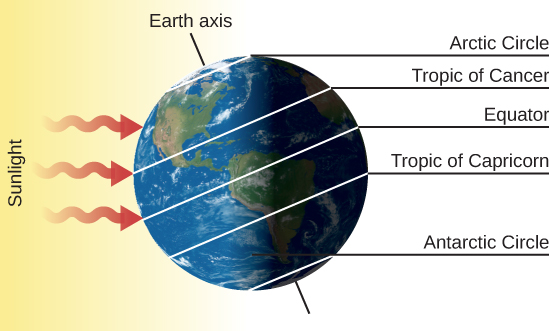
\includegraphics[width=2.5in]{Figures/Figure4.8.jpg}
\end{minipage}
\vspace{1em}

\question
Which astronomical event is depicted in the figure below?

\begin{minipage}{0.45\textwidth}
    \centering
    \begin{choices}
    \choice Spring Equinox\\ (March 21)
    \choice Fall Equinox\\ (September 21)
    \choice Summer Solstice\\ (June 21)
    \correctchoice Winter Solstice\\ (December 21)
    \end{choices}
\end{minipage}%
\begin{minipage}{0.5\textwidth}
    \centering
    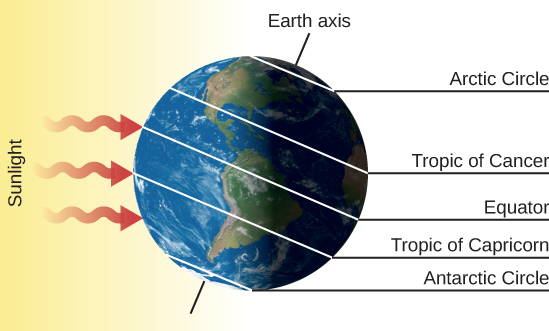
\includegraphics[width=2.5in]{Figures/Figure4.9.jpg}
\end{minipage}
\vspace{1em}

\question
The Tropic of Cancer is at latitude \fillin[][1cm]\ .

\begin{choices}
    \correctchoice \SI{23}{\degree N}
    \choice \SI{0}{\degree} (Equator)
    \correctchoice \SI{23}{\degree S}
    \correctchoice \SI{45}{\degree W}
\end{choices}

\question
If you travel to a place on the Tropic of Cancer (e.g., Hawaii) on the summer solstice, you'll observe that the Sun at noon \ldots

\begin{choices}
    \choice crosses the constellation of Cancer
    \correctchoice is at your zenith (directly overhead)
    \choice reaches its lowest point in the sky
    \choice gets blocked by the Moon
\end{choices}

\question
Which phenomenon is represented in the figure below?
\vspace{1em}

\begin{minipage}{0.4\textwidth}
    \centering
    \begin{choices}
    \choice lunar eclipse
    \choice supernova
    \correctchoice solar eclipse
    \choice retrograde motion
    \end{choices}
\end{minipage}%
\begin{minipage}{0.5\textwidth}
    \centering
    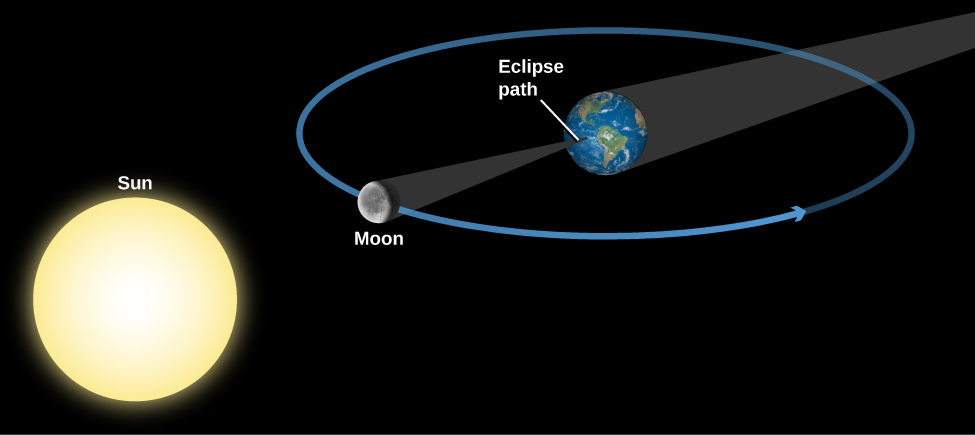
\includegraphics[width=2.5in]{Figures/Figure4.22.jpg}
\end{minipage}
\vspace{1em}

\question
Which part of the Sun may be seen during a solar eclipse? (Warning: never look directly at the Sun).

\begin{choices}
    \choice the core
    \choice the photosphere
    \choice the surface
    \correctchoice the corona (outer atmosphere)
\end{choices}

\question
How long does viewing a solar eclipse last?

\begin{choices}
    \choice about 1 hour
    \correctchoice no more than 7 minutes
    \choice 7 days
    \choice 1 month
\end{choices}

\question
Which phenomenon is represented in the figure below?
\vspace{1em}

\begin{minipage}{0.4\textwidth}
    \centering
    \begin{choices}
    \correctchoice lunar eclipse
    \choice supernova
    \choice solar eclipse
    \choice hypernova
    \end{choices}
\end{minipage}%
\begin{minipage}{0.5\textwidth}
    \centering
    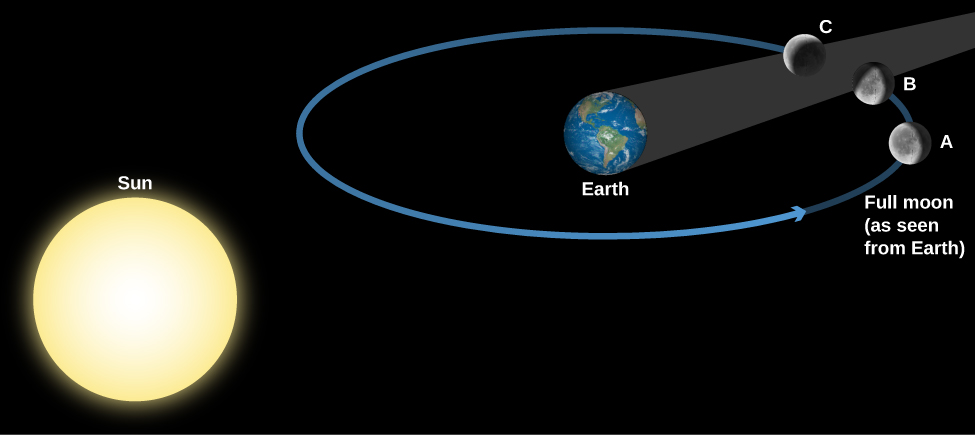
\includegraphics[width=3in]{Figures/Figure4.24.jpg}
\end{minipage}

\question
What happens during a lunar eclipse?

\begin{choices}
    \choice The Moon blocks sunlight on Earth's surface.
    \choice The Moon's atmosphere reflects sunlight, turning it ``blood'' orange.
    \choice The Sun and Moon collide.
    \correctchoice The Earth blocks sunlight on the Moon's surface.
\end{choices}

\question
Why don't lunar and solar eclipses happen every month?

\begin{choices}
    \correctchoice The \SI{5}{\degree} tilt of the Moon's orbit usually prevents the Earth and Moon from crossing each others' shadows.
    \choice The Sun isn't always bright enough to make eclipses happen.
    \choice Eclipses only happen when at least 3 planets in the solar system align.
    \choice They do happen every month; we just can't see them in Texas all the time.
\end{choices}

\question 
What causes the Moon to turn ``blood'' orange during a lunar eclipse?

\begin{choices}
    \choice The Moon's atmosphere absorbs red wavelengths from the Sun.
    \choice The Moon's true orange surface is made visible during an eclipse.
    \correctchoice Earth's atmosphere focuses the redder wavelengths of light on the Moon (like during a sunset).
    \choice The orange light from Mars reflects off the Moon
\end{choices}

\question
Suppose it's been over 3 weeks since the last new moon. You look up at night and see the Moon below. What phase is this?

\begin{minipage}{0.3\textwidth}
    \begin{choices}
        \choice waning gibbous
        \choice waxing gibbous
        \correctchoice waning crescent
        \choice waxing crescent
    \end{choices}
\end{minipage}%
\begin{minipage}{0.3\textwidth}
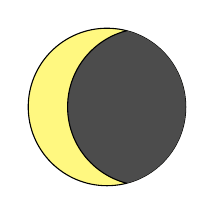
\begin{tikzpicture}
    \draw[fill=yellow!50] (0,0) circle (1cm);
    \begin{scope}
        \clip (0,0) circle (1cm);
        \draw[fill=black!70] (0.5,0) circle (1cm);
    \end{scope}
\end{tikzpicture}
\end{minipage}

\question
Suppose you head about a full moon that will occur in a few days. You look up at night and see the Moon below. What phase is this?

\begin{minipage}{0.3\textwidth}
    \begin{choices}
        \correctchoice waxing gibbous
        \choice waning gibbous
        \choice waxing crescent
        \choice waning crescent
    \end{choices}
\end{minipage}%
\begin{minipage}{0.3\textwidth}
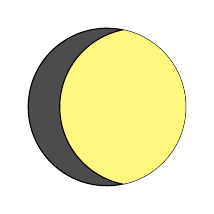
\begin{tikzpicture}
    \draw[fill=black!70] (0,0) circle (1cm);
    \begin{scope}
        \clip (0,0) circle (1cm);
        \draw[fill=yellow!50] (0.4,0) circle (1cm);
    \end{scope}
\end{tikzpicture}
\end{minipage}

\end{questions}
\end{document}



